\documentclass{ximera}

\author{Anna Davis} \title{MTH 160 Quiz 26} 

\begin{document}

\begin{abstract}

\end{abstract}
\maketitle
 \textit{Soft Deadline: April 27, 2020}
\begin{problem}\label{prob:quiz26prob1}
Find the positive degree measure of each angle.
\begin{image}
   
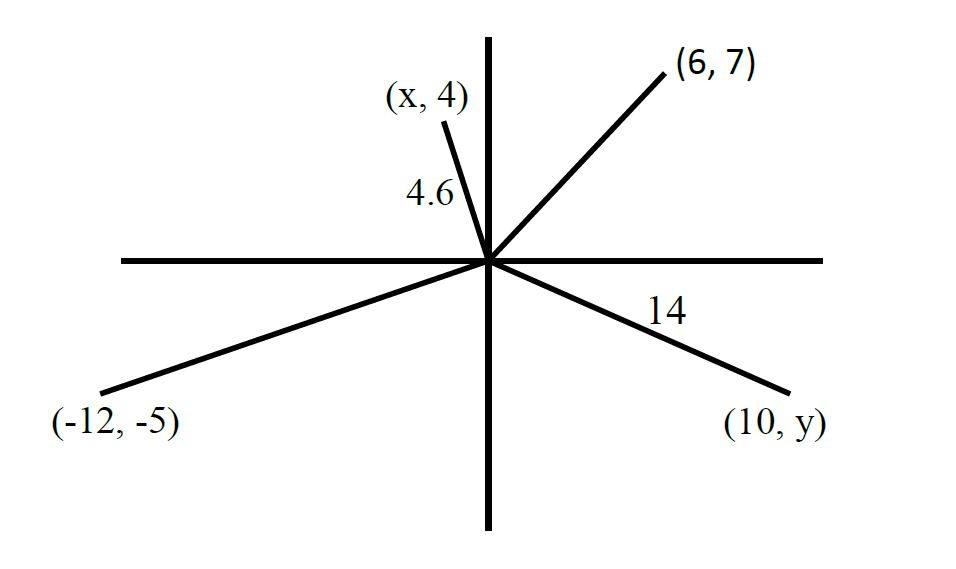
\includegraphics[height=1in]{angles.jpg}~
 
\end{image}

Quadrant I:
$$\answer[tolerance=0.1]{49.4}\mbox{ degrees}$$

Quadrant II:
$$\answer[tolerance=0.1]{119.6}\mbox{ degrees}$$

Quadrant III:
$$\answer[tolerance=0.1]{202.6}\mbox{ degrees}$$

Quadrant IV:
$$\answer[tolerance=0.1]{315.6}\mbox{ degrees}$$

\end{problem}

\end{document} 